% ==========================================================
%
% Dies ist die LaTeX-Datei für das zweite Praxisprojekt von:
%
%                		Fabian Reitz
%
%				       mit dem Titel:
%
%  					 "Praxisprojekt 2"
%					
%			 in Kooperation mit stadt.werk GmbH
%
% ==========================================================



% ----------------------------
%
% Konfiguration des Dokumentes
%
% ----------------------------

% Dokumenten-Klasse und Format auf A4 festlegen:
\documentclass[a4paper]{scrartcl}

% Einen Zähler für Paragraphen benutzen:
\addtocounter{tocdepth}{1}

% Einrückung bei Absatzbeginn verhindern:
\setlength{\parindent}{0pt}



% ------------------
%
% Benötigte Packages
%
% ------------------

% Europäisches Buchstaben-Encoding verwenden:
\usepackage[T1]{fontenc}
\usepackage{csquotes}

% Deutsche Rechtschreibung nach aktueller Reform verwenden:
\usepackage[ngerman]{babel}

% Fontspec verwenden:
\usepackage{fontspec}

% Zeilenabstand verwenden:
\usepackage{setspace}

% Abschnitte im Dokument verlinken: 
\usepackage{hyperref}
\hypersetup{
	pdfencoding=auto,
	pdftitle={TITEL},
	pdfsubject={THEMA},
	pdfauthor={Fabian Reitz},
	pdfkeywords={},
   	hidelinks
}

% Befehle zum Festlegen der aktuellen Uhrzeit verwenden:
\usepackage{scrtime}

% Einbinden von Grafiken:
\usepackage{graphicx}
\usepackage{float}
\usepackage{sidecap}

% Setzen der Seitenabstände
\usepackage[a4paper, left=4cm, right=4cm, top=3cm, bottom=1.5cm]{geometry}

% Ein Abkürzungsverzeichnis benutzen:
\usepackage{acronym}

% Den Header des Dokumentes bearbeiten:
\usepackage{fancyhdr}

% Inhaltsverzeichnis und Abbildungsverzeichnis in 
% das Inhaltsverzeichnis einbinden:
\usepackage[notbib]{tocbibind}

% Setzen von Punkten als Trenner in das Inhaltsverzeichnis:
\usepackage[titles]{tocloft}
\renewcommand{\cftsecleader}{\cftdotfill{\cftdotsep}}

\usepackage{tocloft}

\setlength{\cftbeforesecskip}{3pt}

\usepackage{makecell}

\usepackage{titlesec}

\setcounter{secnumdepth}{4}

\titleformat{\paragraph}
{\normalfont\normalsize\bfseries}{\theparagraph}{1em}{}
\titlespacing*{\paragraph}
{0pt}{3.25ex plus 1ex minus .2ex}{1.5ex plus .2ex}

\usepackage{amsmath}

\usepackage{chngpage}

% --------------------------------
%
% Einstellungen für die Schriftart
%
% --------------------------------

% Schriftart auf "Times New Roman" festlegen:
\setmainfont[
	Path = ./fonts/,
    BoldFont = Times-New-Roman-Bold.ttf,
    ItalicFont = Times-New-Roman-Italic.ttf
]{Times-New-Roman.ttf}

% Header bearbeiten:
\pagestyle{fancy}
\fancyhf{}
\fancyhead[C]{- \thepage\ -}
\renewcommand{\headrulewidth}{0pt}

\linespread{1.5}


% ---------------------
%
% Anfang des Dokumentes
%
% ---------------------

\begin{document}


% ---------------------
% Deckblatt definieren:
% ---------------------



\titlehead{\centering
\includegraphics[scale=0.3]{assets/logo_DHSH}}
\subject{Praxisprojekt 2 - Informatik \\}
\title{Der Nutzen von digitalem Wissensmanagement in mittelständischen IT-Unternehmen \\ - am Beispiel einer digitalen Bibliothek}

\author{\date{}}
\vspace{2cm}
\publishers{
	\begin{tabbing}
		Betreuender Dozent: tab \= Mitte \= Rechts \= \kill
		
		Abgegeben von: 	\> Fabian Reitz \\
		E-Mail: 		\> fabian.reitz@stud.dhsh.de \\
		Studiengruppe:	\> WINF 119 B \\ \\
		Gutachter:		\> Herr Prof. Dr. Alexander Paar \\ \\
		Abgabetermin:	\> 29.04.2021 \\
		Versuch:		\> Erstversuch \\
	\end{tabbing}
}
\maketitle

\thispagestyle{empty}



% -------------------
% Inhaltsverzeichnis:
% -------------------

\newpage

% Alle folgenden Seiten in römischen Zahlen zählen:
\pagenumbering{Roman}

% Beginn der Paginierung bei zwei:
\setcounter{page}{2}

% Inhaltsverzeichnis zeigen:
\tableofcontents


% ----------------------
% Abkürzungsverzeichnis:
% ----------------------

% Neue Seite beginnen:
\newpage

\section*{Abkürzungsverzeichnis}

\addcontentsline{toc}{section}{Abkürzungsverzeichnis}

% Abkürzungsverzeichnis beginnen:
\begin{tabbing}
	----------------------- \= Erklärung \kill
	API \> Application Programming Interface \\
	\> deutsch: Programmierschnittstelle \\
	GmbH \> Gemeinschaft mit beschränkter Haftung \\
	HDD \> Hard Drive Disk \\
	\> deutsch: Festplatte, magnetisches Speichermedium  \\
	HTTP \> Hypertext Transfer Protocol \\
	\> deutsch: Hypertext-Übertragungsprotokoll \\
	HTTPS \> Hypertext Transfer Protocol Secure \\
	\> deutsch: sicheres Hypertext-Übertragungsprotokoll \\
	IT \> Informationstechnologie \\
	JSON \> JavaScript Object Notation \\
	KQL \> Kibana Query Language \\
	TF/IDF \> Term Frequency - Inverse Document Frequency \\
	\> deutsch: Termfrequenz - Inverse Dokumentfrequenz \\
	TSL \> Transport Layer Security \\
	\> deutsch: Sicherheit auf Ebene der Schnittstellen-Kommunikation \\
	XML \> Extensible Markup Language \\
\end{tabbing}


% ----------------------
% Abbildungsverzeichnis:
% ----------------------
\newpage

\listoffigures


% --------------------
% Tabellenverzeichnis:
% --------------------
\newpage

\listoftables

% -----------
% Einleitung:
% -----------

% Neue Seite erstellen:
\newpage

% Paginierung mit eins beginnen:
\setcounter{page}{1}

% Alle folgenden Seiten in arabischen Zahlen zählen:
\pagenumbering{arabic}

% Neue Section: Einleitung
\section{Einleitung}
Das 21. Jahrhundert steht im Zeichen der digitalen Informationsexplosion. Während in dem Jahr 1984 3,65 Mio. Festplatten des Typs HDD verkauft wurden, wuchs diese Zahl im Jahr 2000 um mehr als 5.400 \% auf 200,1 Mio. verkaufte Einheiten an. Dieser Trend gipfelte im Jahr 2010 bei einer Menge von 651.32 Mio. Stück (Alsop 2020). Der Bedarf, Informationen zu sichern, wächst ununterbrochen. Auch Unternehmen haben ein Interesse daran, Informationen in Form von Wissen zu verwalten. Auf die Frage, wie wichtig die Bedeutung von Wissensmanagement für die deutsche Wirtschaft ist, stimmen 91 \% von 532 befragten Personen mit sehr wichtig bis wichtig (Decker et al. 2005: 28). \\ \\
In diesem Kontext muss die Frage beantwortet werden, wo der Unterschied zwischen Wissen und Informationen liegt. „Wissen bezeichnet die Gesamtheit der Kenntnisse und Fähigkeiten, die Individuen zur Lösung von Problemen einsetzen.“ (Probst et al. 2006: 22). Wissen baut auf Informationen und Daten auf, ist aber an Individuen gebunden. Informationen und Daten können auch ohne Zusammenhang mit Personen existieren. Um diese Definition auf den betrieblichen Kontext auszuweiten, wird der Begriff organisationale Wissensbasis eingeführt. Diese besteht aus Wissensbeständen von einzelnen Mitarbeitenden und dem kollektivem Wissen von Gruppen. Unternehmen können zur Lösung ihrer Aufgaben auf die Wissensbasis zugreifen und somit theoretisch das gesamte kombinierte Wissen der Individuen in einem Unternehmen nutzen (Probst et al. 2006: 22). \\ \\
Im Rahmen dieser Arbeit wird ein besonderes Augenmerk auf die praktische Umsetzung einer digitalisierten organisationalen Wissensbasis gelegt. Ziel dieser Arbeit ist das Erstellen einer digitalen indexierten Bibliothek. Weiterhin wird die Performanz dieser Bibliothek anhand verschiedener komplexer Suchanfragen dargestellt. \\
Zu der Erstellung dieser organisationalen Wissensbasis werden moderne Web-, Datenbank- und Containertechnologien verwendet. Es wird darauf eingegangen, warum speziell diese Technologien verwendet werden und wo die Vorteile zu anderen Technologien liegen.

\newpage

\section{Theoretischer Hintergrund}
Das besondere Augenmerk dieser Arbeit liegt auf dem Aspekt der Informatik, jedoch wird etwas betriebswirtschaftlicher Hintergrund benötigt, um die Relevanz für das Unternehmen zu verdeutlichen. Im Folgenden wird auf wichtige Aspekte beider Bereiche eingegangen, um Unklarheiten zu beseitigen und grundsätzliches Wissen für die spätere Umsetzung des Projektes zu vermitteln.

\subsection{stadt.werk}
Das Projekt der Schaffung einer digitalisierten organisationalen Wissensbasis wird mithilfe des Unternehmens stadt.werk konzeption.text.gestaltung GmbH durchgeführt. Zur Reduzierung der Wortwahl und aus Gründen der Lesbarkeit wird das Unternehmen im Folgenden als stadt.werk abgekürzt. Das Unternehmen gehört per Definition der Gruppe der Dienstleistungsbetriebe an (Wöhe 2010: 31) und erstellt Software nach dem Prinzip software-as-a-service (Benlian und Hess 2011: 232). stadt.werk beschäftigt aktuell elf Mitarbeitende und zwei Geschäftsführer. Nach der Definition der Europäischen Kommission ist stadt.werk der Gruppe der KMU zuzuordnen. In dieser Kategorie ist das Unternehmen per Definition ein kleines Unternehmen, da es einen Jahresumsatz von 10 Mio. EUR und eine Obergrenze von 50 Beschäftigten nicht überschreitet (EU-Kommission 2003: 39). \\
Das Unternehmen stadt.werk ist eine Tochtergesellschaft des Landwirtschaftlichen Buchführungsverbandes, welcher gleichzeitig der bedeutendste Kunde des Unternehmens ist. Die Spezialisierung stadt.werks liegt dabei in der Schaffung und Wartung von Intranetsystemen auf der Basis von Webtechnologien.

\subsection{Wissensmanagement}

\subsubsection{Bedeutung von Wissensmanagement}
Der Wunsch, Wissen zu verwalten und zugänglich zu machen, ist nicht neu. Technologien mit einem Alter von mehr als 2000 Jahren zeigen, dass die Bewahrung und Weitergabe von Wissen schon lange eine wichtige Rolle im Leben der Menschen spielt (Moore 2000, zitiert nach Decker et al. 2005: 15). Der Drang danach, Wissen zu managen, in Kombination mit der eingangs erwähnten Informationsexplosion, stellt Unternehmen des 21. Jahrhunderts vor eine große Aufgabe. Es muss eine Möglichkeit gefunden werden, Wissen skalierbar, digital und möglichst schnell jederzeit zugänglich zu machen. \\
Es lässt sich jedoch die Frage stellen, wozu Wissensmanagement benötigt wird. Angenommen, eine beschäftigte Person besitzt viel Wissen über unternehmensinterne Abläufe. Behält sie dieses Wissen für sich und bringt es nicht in eine organisationale Wissensbasis ein, macht sich diese Person zwar unverzichtbar für das Unternehmen, jedoch macht dieses Verhalten ein Unternehmen langsam und unflexibel. Sollte dieser Person theoretisch etwas zustoßen, wäre ein bedeutender Teil des Wissens über das Unternehmen verloren. \\
Führungskräfte haben ein besonderes Interesse daran, Wissensmanagement in den Unternehmen umzusetzen. Das Sammeln und Verwalten von Wissen hilft Führungskräften, einen besseren, dezentralisierten Umgang mit dieser wichtigen Ressource zu gewährleisten (Probst et al. 2006: 22). Der rasante Fortschritt der Informationstechnologie in Zusammenhang mit dem Fortschritt in der Computertechnik ermöglichte seit den 1990er Jahren eine umfassende Wissensbewahrung und einen schnellen Zugriff auf Informationen aller Art (Decker et al. 2005: 14). „Für zahlreiche Unternehmen rückte das Management von Wissen in den Mittelpunkt der Betrachtung.“ (Decker et al. 2005: 14).

\subsubsection{Wissensmanagement im aktuellen Kontext}
Die Ende 2019 ausgebrochene Lungenkrankheit COVID-19 stellt das öffentliche und private, aber auch das betriebliche Leben vor neuartige Herausforderungen. Kontakt- und Zugangsbeschränkungen traten in Kraft, sodass die bisherige Arbeit aus dem herkömmlichen Büro nicht länger möglich ist. Mitarbeiterinnen und Mitarbeitern mussten Möglichkeiten eingeräumt werden, ihrer Arbeit aus den eigenen vier Wänden nachzugehen. Wissen in Form von physischen Büchern in den Schränken der Unternehmen ist nicht länger einfach zugänglich.

\subsection{Elasticsearch}
Die Umsetzung des Projektes erfolgt mit der Suchmaschinen- und Datenbanktechnologie Elasticsearch. Sie ermöglicht das Durchsuchen von beispielsweise Textdaten, numerischen Daten und Geodaten. Die häufige Nutzung von Elasticsearch zeigt sich in vielen theoretischen und praktischen Beispielen. So kann Elasticsearch bei der Suche in Anwendungen, auf Websites, in Unternehmensdaten, aber auch beim Logging von Anwendungen und der Analyse dieser Logs dienen (Was ist Elasticsearch?, o.D.). Auch in der Praxis nutzen Unternehmen Elasticsearch. Darunter fallen beispielsweise Wikipedia, Stack Overflow, GitHub (Gormley und Tong 2015: 1) und mittelständische Unternehmen wie beispielsweise stadt.werk. \\
Elasticsearch wurde in Java programmiert und basiert auf Lucene. Erst Lucene ermöglicht es, die Datensätze in Elasticsearch zu indexieren und durchsuchbar zu machen (Gormley und Tong, 2015: 3). Im Kontext dieser Arbeit wird auf eine genauere Erklärung von Lucene verzichtet.


\subsubsection{Elasticsearch als Datenbanksystem}
Elasticsearch bedient sich eines dokumentenorientieren Ansatzes und zählt so zu der Gruppe der sogenannten NoSQL-Datenbanken (Meier und Kaufmann 2016:18). Die wesentlichen Unterschiede zwischen Elasticsearch und relationalen Datenbanksystemen nach Edgar Frank Codd werden in einem späteren Abschnitt aufgezeigt. 

\paragraph{Dokumentenorientierte Datenbanksysteme}
Dokumentenorientierte Datenbanksysteme bedienen sich eines einfachen Schlüssel-Wert-Prinzips (englisch: key-value), wie es sich auch in dem Format JSON findet. Demnach kann jedem Schlüssel ein Wert zugewiesen werden. Diese Schlüssel-Wert-Paare bilden ein Objekt. Es ist möglich, von einem Schlüssel auf den entsprechenden Wert zuzugreifen. Während die Schlüssel dem Datentyp String entsprechen, kann der zugehörige Wert jeden Datentyp annehmen, beispielsweise Number, String, Array oder Objekt. So ist eine tiefe Verschachtelung möglich. Ein forciertes Schema ist nicht notwendig, kann jedoch bei Bedarf Anwendung finden (Pezoa et al. 2016: 263f).

\paragraph{Aufbau von Elasticsearch}
Wird ein erstelltes Objekt in einer NoSQL-Datenbank wie Elasticsearch gesichert, bildet jedes Schlüssel-Werte-Paar dieses Objekts die kleinste Entität einer dokumentenorientierten Datenbank. Diese Entität wird Feld genannt (Gormley und Tong 2015: 10-11). \\

Das gesicherte Objekt, bestehend aus beliebig vielen Feldern, bezeichnet man als Dokument. Alle Felder eines Dokuments beziehen sich auf eine felderübergreifende Entität und beschreiben diese (Gormley und Tong 2015: 10f). \\

Beliebig viele Dokumente, die ähnliche oder vergleichbare Entitäten beschreiben, werden in sogenannten Typen zusammengefasst (Gormley und Tong 2015: 10f). \\

Beliebig viele Typen werden in einem Index gesichert (Gormley und Tong 2015: 10f). \\

Eine Instanz von Elasticsearch kann beliebig viele Indizes unterhalten (Gormley und Tong 2015: 10f). \\ \\
Die beschriebene hierarchische Struktur lässt sich durch die folgende Abbildung vereinfacht darstellen.

\begin{figure}[h!]
	\centering
	\caption{Aufbau von Elasticsearch als Datenbanksystem}
	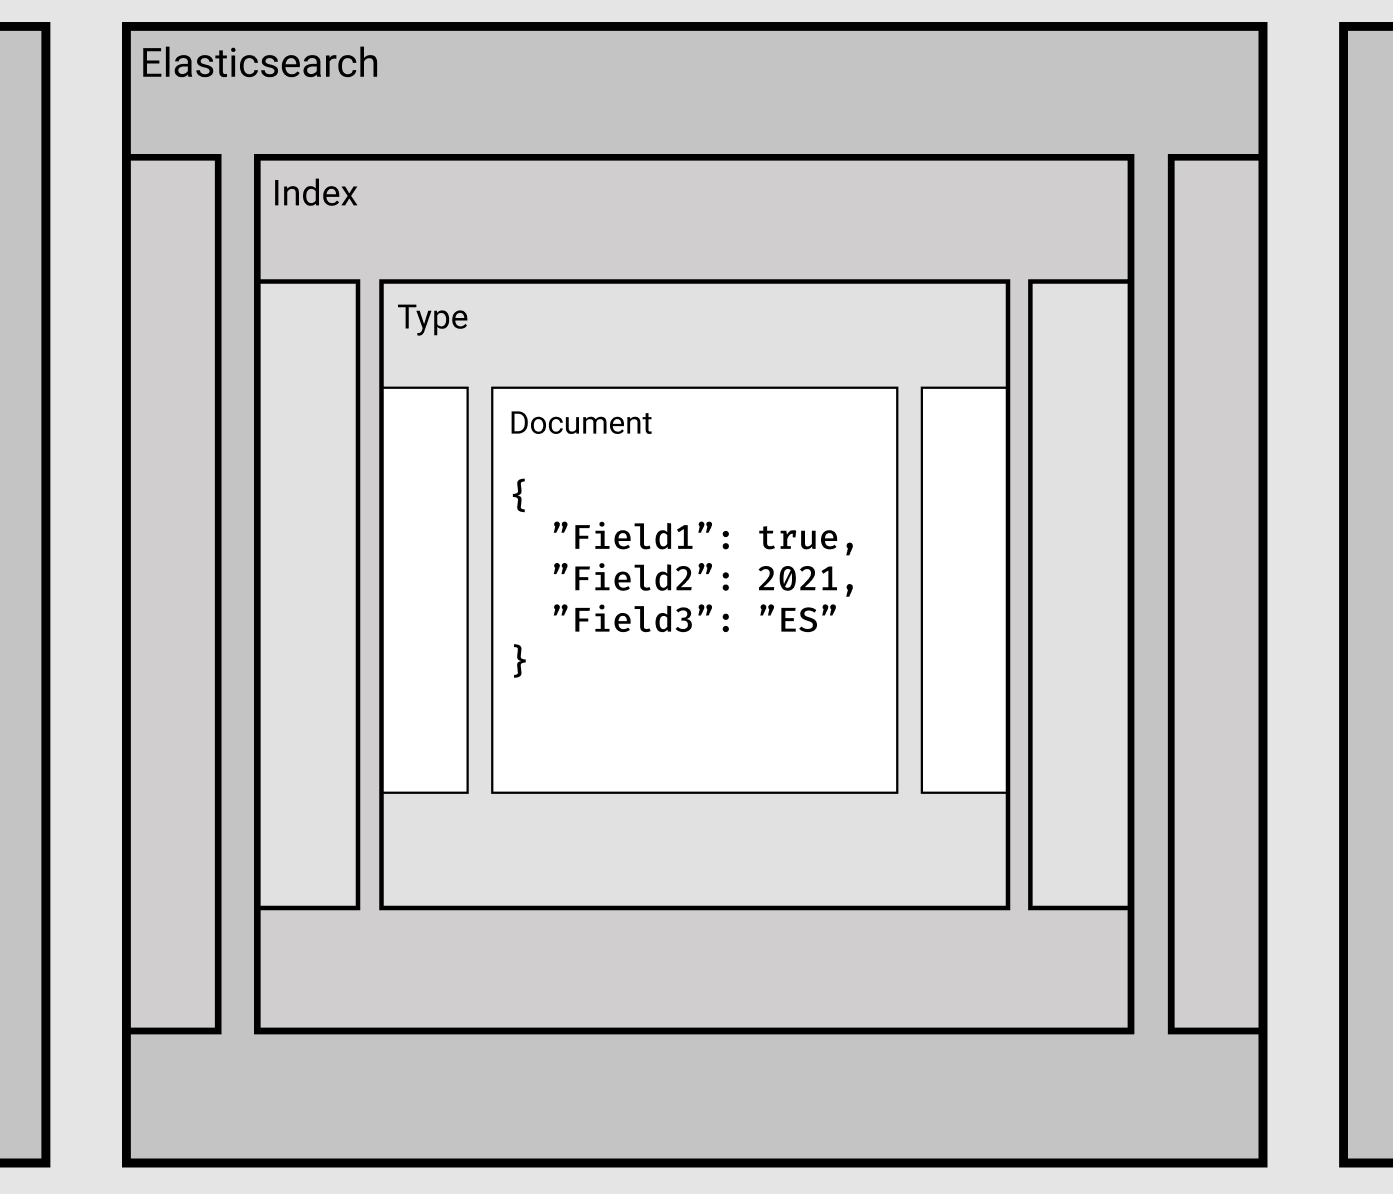
\includegraphics[scale=0.2]{assets/Elasticsearch_Structure} \\
	Die hier gezeigte Abbildung stellt vereinfacht den Aufbau und die Hierarchie von Elasticsearch dar. Es ist erkennbar, dass jede gezeigte Entität mehrfach vorkommen kann.
\end{figure}
   
    
\subsubsection{Vergleich mit relationalen Datenbanksystemen}
Für einen Vergleich zwischen relationalen und dokumentenorientierten Datenbanksystemen muss zunächst eine Einordnung von relationalen Datenbanksystemen erfolgen. Durch das verhältnismäßig hohe Alter dieser Technologie gibt es viele Punkte zu den Themen Geschichte, Entwicklung, Algebra und Ausprägungen zu beachten. Da das Beleuchten all dieser Themen den Umfang dieser Arbeit überschreiten würde, werden diese Punkte lediglich kurz und beispielhaft dargestellt.

\paragraph{Einordnung relationaler Datenbanksysteme}
Um Daten und Informationen einfach und übersichtlich aufzuzeigen, eignet sich die Darstellung als Tabelle. Eine Tabelle besteht aus Zeilen und Spalten, die kleinste Entität bildet die Zelle. Bestückt man die Spalten der Tabelle mit Merkmalen, lassen sich pro Zeile, sogenannte Tupel, verschiedene Einträge persistieren. Dabei folgt jedes Tupel einem Schema, bestehend aus den vorher festgelegten Merkmalen. Ein Merkmal kann zur eindeutigen Identifizierung eines Tupels als Schlüsselmerkmal dienen. Dieser Identifikationschlüssel muss einmalig sein, um die Eindeutigkeit zu gewährleisten. Sollte ein Schlüssel aus einer Kombination von Merkmalen bestehen, müssen diese minimal sein. Es darf kein Merkmal der Kombination gestrichen werden. Demnach lassen sich die zwei Grundsätze Eindeutigkeit und Minimalität festhalten. Sind diese Grundsätze erfüllt, ist ein Identifikationsschlüssel vollständig charakterisiert (Meier und Kaufmann 2016: 3ff). \\
Es bleibt zu bemerken, dass die Anzahl der Merkmale und der Tupel beliebig sein kann, auch ihre Reihenfolge ist bedeutungslos (Meier und Kaufmann 2016: 6). \\ \\
Die bisher definierte Einordnung umfasst lediglich Daten in Form einer Tabelle. Um relationale Datenbanksysteme grundsätzlich verstehen zu können, muss das Relationenmodell Erwähnung finden. Das Relationenmodell wurde in den 1970er Jahren von Edgar Frank Codd begründet. Es stellt Beziehungen zwischen den Daten von Tabellen dar und stellt diese wiederum tabellarisch dar. Demnach ist eine Relation eine „[...] Teilmenge aus dem kartesischen Produkt von Wertebereichen [...]“ (Meier und Kaufmann 2016: 6). Folgendes Beispiel wird von Meier und Kaufmann gegeben:
\begin{center}
	„$ R \subseteq D \textsubscript{1} \times D \textsubscript{2} \times ... \times D \textsubscript{n} $
	mit $ D \textsubscript{i} $ als Wertebereich des i-ten Attributs resp. Merkmals. “ (2016: 6)
\end{center}
Das Relationenmodell erlaubte die Entstehung erster relationaler Datenbanksysteme, die SQL als Datenbanksprache unterstützen (Meier und Kaufmann 2016: 6). Relationale Datenbanksysteme lassen sich durch die Eigenschaften Modell, Schema, Sprache, Architektur, Mehrbenutzerbetrieb, Konsistenzgewährung und Datensicherheit beschreiben (Meier und Kaufmann 2016: 10). In den folgenden Abschnitten werden diese kurz beschrieben.

\subparagraph{Modell}
Das Relationenmodell ist für relationale Datenbanken von unabdingbarer Wichtigkeit. Es beschreibt die Voraussetzung, dass alle Daten und Datenbeziehungen tabellarisch dargestellt werden. Abhängigkeiten zwischen Tupeln oder mehrfach vorkommende Merkmale können so aufgedeckt werden (Meier und Kaufmann 2016: 10).

\subparagraph{Schema}
Das relationale Datenbankschema beschreibt die Tabellen und deren Merkmale. Durch das Schema wird der Informationsgehalt der Tupel vergleichbar und die Merkmale werden forciert. Weiterhin enthält ein Schema die Beschreibung der Schlüsselmerkmale und Regeln zur Sicherstellung der Integrität (Meier und Kaufmann 2016: 10). Integrität bezeichnet im Kontext von relationalen Datenbanken die Einigkeit und Widerspruchsfreiheit von Daten. Sie ist erreicht, wenn Daten korrekt erfasst werden. Sie gilt als verletzt, wenn Mehrdeutigkeiten oder Widersprüche auftreten (Meier und Kaufmann 2016: 56).

\subparagraph{Sprache}
Die Datenbanksprache SQL dient dem Datenbanksystem zur Definition, Selektion und Manipulation von Daten (Meier und Kaufmann 2016: 10). Auf weitere Erläuterungen zu SQL als Datenbanksprache wird im Kontext dieser Arbeit bewusst verzichtet.

\subparagraph{Architektur}
Ein relationales Datenbanksystem zielt auf eine möglichst hohe Datenunabhängigkeit ab. So bleiben Datenbanksystem und Anwendungsprogramme bestenfalls voneinander getrennt. Eine händische Änderung an den Daten kann vorgenommen werden, ohne dass Anpassungen an den Anwendungsprogrammen nötig sind (Meier und Kaufmann 2016: 10). \\
Im Themenbereich der Softwarearchitektur findet sich das vergleichbare Prinzip Model-View-Controller wieder. Auch hier gilt eine Trennung von Datenbestand, User Interface und Programmlogik als erstrebenswert (Deacon 2009: 1f). 

\subparagraph{Mehrbenutzerbetrieb}
Das Datenbanksystem erlaubt die gleichzeitige Nutzung durch mehrere Nutzer. Sie können eine Datenbank parallel abfragen oder verändern, ohne dass gegenseitige Behinderungen erfolgen oder die Integrität verletzt wird (Meier und Kaufmann 2016: 11).

\subparagraph{Konsistenzgewährung}
Wie bereits erwähnt, stellt ein Datenbanksystem dem Nutzer Möglichkeiten zur Verfügung, um die Integrität der Daten sicherzustellen. Somit wird die Konsistenz der Daten garantiert (Meier und Kaufmann 2016: 11).

\subparagraph{Datensicherheit}
Das Datenbanksystem bietet Möglichkeiten, die Daten vor Zerstörung, Verlust oder unbefugtem Zugriff zu sichern (Meier und Kaufmann 2016: 11). Zu diesen Möglichkeiten zählt beispielsweise das Einrichten von Views. Dem Nutzer wird so nur die Tabelle oder der Tabellenausschnitt gezeigt, für dessen Einsicht er berechtigt ist (Meier und Kaufmann 2016: 128). \\ 

Datenbanksysteme, welche nicht den relationalen Ansatz verfolgen, erfüllen die genannten Eigenschaften nur teilweise.

\paragraph{Gemeinsamkeiten zwischen Elasticsearch und relationalen Datenbanksystemen}
Blickt man auf die Definitionen der beiden Datenbankprinzipien, fällt auf, dass relationale Datenbanksysteme vielen Eigenschaften von unabdingbarer Wichtigkeit folgen. Einige dieser Eigenschaften finden sich in Elasticsearch wieder, wobei diese zum Teil optionaler Natur sind. Im Folgenden wird auf Eigenschaften eingegangen, die Parallelen und Ähnlichkeiten zwischen Elasticsearch und dem relationalen Datenbankprinzip aufzeigen. \\

Der Aufbau von Elasticsearch ähnelt dem einer relationalen Datenbank. Die Parallelität der Ebenen beider Systeme kann durch folgende Tabelle verdeutlicht werden.

\begin{table}[htb]
	\centering
	\caption{Vergleichbare Ebenen von Elasticsearch und relationalen Datenbanksystemen}
	\begin{center}
		
		\begin{tabular}{|c||c | c|}
			\hline
			Ebenen & Elasticsearch & relationale Datenbanksysteme \\ [0.5ex]
			\hline \hline
			-1 & Indizes & Datenbanken \\
			\hline
			-2 & Typen & Tabellen \\
			\hline
			-3 & Dokumente & Tupel \\
			\hline
			-4 & Felder & Merkmale \\
			\hline
		\end{tabular}
	\end{center}
	Die Tabelle zeigt die Ebenen der zu vergleichenden Systeme. Ebene 0 steht für das System. Je kleiner die identifizierende Zahl der Ebene, desto tiefer die Ebene. Die Ebene -4 symbolisiert die kleinste Entität des jeweiligen Systems. Der Vergleich dient der Orientierung und der Einordnung (Gormley und Tong 2015: 10f).
\end{table}

Vergleicht man mehrere Tupel einer relationalen Datenbank mit den Dokumenten von Elasticsearch, fällt auf, dass Dokumente nicht zwangsweise einem forcierten Schema folgen. Dokumente in einem Typ können je nach Anforderung individuell gestaltet sein. Sollte doch Bedarf nach einem forcierten Schema entstehen, bietet Elasticsearch einen Prozess mit der Bezeichnung Mapping an (Gormley und Tong 2015: 87f). \\
Mapping bezeichnet das Forcieren eines Schemas für einen Typ in einem Index. Dieses Schema findet bei allen Dokumenten dieses Typs Anwendung. Das Mapping bestimmt so die Felder in einem Dokument, den Datentyp eines Feldes und wie dieses Feld von Elasticsearch behandelt wird (Gormley und Tong 2015: 87f). \\

Betrachtet man die Grundsätze der Architektur beider Systeme, lassen sich auch hier Ähnlichkeiten feststellen. Eine strikte Trennung der Datensätze und der Anwendungslogik wird im Kontext von Elasticsearch durch verschiedene Programmierschnittstellen (engl. APIs) gewährleistet. So ist es möglich, dass die Anwendungslogik mithilfe von JSON und HTTP mit Elasticsearch kommunizieren kann und die Daten einlesen oder anpassen kann. Diese APIs ermöglichen, dass die Sprache der Anwendungslogik unwichtig ist, solange diese JSON und HTTP unterstützen (Gormley und Tong 2015: 7). \\

Elasticsearch unterstützt die Nutzung durch mehrere Nutzer. Überprüfbar ist dies beispielsweise mit dem Feld \texttt{\_version} eines Dokuments. Jedes Dokument besitzt dieses Feld, es zählt zu seinen Metadaten. Das Feld besitzt den Datentyp Integer und wird bei Änderungen durch einen Nutzer inkrementiert (Gormley und Tong 2015: 48). Sollte ein Dokument zwei Änderungsanfragen erhalten, kann durch dieses Feld erkannt werden, welche Änderung zuletzt kam und damit den Inhalt des Dokuments verändert hat. \\

Die Konsistenzgewährung ist ebenfalls durch Elasticsearch gegeben. Durch sogenannte Shards und Replicasets werden Mechanismen bereitgestellt, die Hardwareausfällen und Integritätsverletzungen vorbeugen können (Gormley und Tong 2015: 25). \\

Die Datensicherheit kann im Kontext von Elasticsearch über Nutzerkonten für die Oberfläche Kibana ermöglicht oder optional über zusätzliche Sicherheitsstufen auf Ebene der APIs gewährleistet werden. Dabei findet TSL und HTTPS besondere Erwähnung (Configure security for the Elastic Stack, o.D.). Weiterhin ermöglicht Elasticsearch durch die bereits erwähnten Technologien Shards und Replicaseats einen hohen Schutz vor Datenverlust. \\ 

Während Elasticsearch einige Ähnlichkeiten zu dem grundlegenden Konzept relationaler Datenbanksysteme besitzt, sollte jedoch Erwähnung finden, dass hier Elasticsearch als konkrete Ausprägung einer NoSQL-Datenbank mit den grundlegenden Konzepten von relationalen Datenbanken verglichen wird. Individuelle Ausprägungen relationaler Datenbanksysteme weisen unter Umständen mehr oder weniger Gemeinsamkeit auf.

\paragraph{Unterschiede zwischen Elasticsearch und relationalen Datenbanksystemen}
Der Grundlegende Unterschied zwischen diesen beiden Datenbanksystemen zeigt sich in dem relationalen Ansatz relationaler Datenbanken und dem dokumentenorientieren Ansatz von Elasticsearch. Daten und Information werden in Elasticsearch nicht in Tabellen, sondern in Dokumenten gespeichert. \\

Die Anfragen gegen Elasticsearch werden nicht mit der Datenbanksprache SQL formuliert. Werden Anfragen von einem Programm erstellt, werden die APIs von Elasticsearch angefragt. Diese Anfrage geschieht mithilfe von HTTP oder HTTPS. Dabei kann auf die Methoden GET, POST, PUT, HEAD und DELETE zurückgegriffen werden (Gormley und Tong 2015: 7). In vielen Fällen bietet Elasticsearch Clients für die jeweilige Programmierumgebung an. Als Beispiel sei hier Node.js und der Elasticsearch-Client für Node.js aufgeführt (Elasticsearch Node.js client, o.D.). \\
Sollte ein Entwickler direkte Anfragen gegen Elasticsearch stellen wollen, bieten sich ihm zwei Möglichkeiten. Einerseits kann er HTTP-Anfragen mittels Programmen wie cURL oder Postman stellen. Dabei werden ebenfalls die APIs von Elasticsearch angesprochen (Gormley und Tong 2015: 7). Die zweite Möglichkeit umfasst die Nutzung von Kibana. Kibana ist ein umfangreiches Programm zur Darstellung und Visualisierung von Daten in Elasticsearch. Darüber hinaus bietet Kibana die Möglichkeit, Anfragen gegen Elasticsearch zu stellen (Ihr Fenster in den Elastic Stack, o.D.). Kibana nutzt dafür die Datenbanksprache KQL, die dem Syntax von cURL ähnlich ist (Kibana Query Language, o.D.). \\

Auch hier muss Erwähnung finden, dass die grundlegenden Konzepte relationaler Datenbanksysteme mit Elasticsearch als konkrete Ausprägung eines NoSQL-Datenbanksystems verglichen werden. Individuelle Ausprägungen des relationalen Datenbankkonzeptes weisen unter Umständen mehr oder weniger Ähnlichkeit auf. Des Weitern muss besonders berücksichtigt werden, dass Elasticsearch keine reine dokumentenorientierte Datenbank ist. Elasticsearch erweitert die Prinzipien einer dokumentenorientierten Datenbank um die Möglichkeiten, die Daten mittels Lucene zu indexieren und durchsuchbar zu machen. Als Beispiel für eine reine dokumentorientierte Datenbank sei hier MongoDB erwähnt.

\subsubsection{Elasticsearch als Suchmaschine}
Wie bereits erwähnt, ist Elasticsearch mehr als nur ein dokumentenorientiertes Datenbanksystem. Es bietet dank Lucene die Möglichkeiten, Daten zu indexieren und durchsuchbar zu machen (Gormley und Tong 2015: 38). Da der Begriff Index im Kontext von Elasticsearch mehrfach benutzt wird, folgen kurze Definitionen zu dem Begriff Index.

\subparagraph{Der Index}
Der Index von Elasticsearch beschreibt einen Ort, an welchem Dokumenten gespeichert werden, die in einem Zusammenhang stehen. Er ist mit den Datenbanken eines relationalen Datenbankmodells vergleichbar (Gormley und Tong 2015: 11). Die übergeordnete Entität bildet das System Elasticsearch und die untergeordneten Entitäten werden durch Typen beschrieben. Es besteht die Möglichkeit, dass Elasticsearch mehrere Indizes unterhält (Gormley und Tong 2015: 10f).

\subparagraph{Indexieren}
Ein Dokument wird indexiert, wenn es in einem Index gesichert wird. Auf diese Weise kann das Dokument durchsucht und angefragt werden (Gormley und Tong 2015: 11).

\subparagraph{Der inventierte Index}
Der invertierte Index ist eine von Elasticsearch genutzte Methode, um schnelle Volltextsuchen zu ermöglichen. Dazu werden alle einzigartigen Wörter von jedem Dokument in einer geordneten Liste gesichert und normalisiert. Normalisieren bedeutet in diesem Kontext, dass die Wörter als klein geschriebene Strings gesichert und auf ihren Wortstamm beschränkt werden. Zusätzlich zu dieser Liste wird eine weitere Liste von Dokumenten erstellt, in welchen die Wörter der ersten Liste vorkommen (Gormley und Tong 2015: 81). Im Folgenden wird der Prozess der Erstellung eines invertierten Indexes vereinfacht definiert. \\
Um einen invertierten Index von beliebig vielen Dokumenten zu erstellen, wird zunächst der Wert eines jeden Feldes eines jeden Dokumentes gesichert. Sollte dieser Wert ein String bestehend aus mehreren Wörtern sein, werden diese einzeln in der eingangs erwähnten Liste gesichert und normalisiert. Die Einträge dieser Liste werden im Kontext von Elasticsearch Terme genannt. Zusätzlich wird gesichert, in welchem Dokument diese Terme vorkommen (Gormley und Tong 2015: 81ff). \\
Angenommen es werden zwei Dokumente indexiert. Diese enthalten jeweils ein Feld mit der Bezeichnung \texttt{inhalt}. Der Wert dieses Feldes ist vom Typ String und wird beispielhaft in folgender Tabelle aufgezeigt. 

\begin{table}[htb]
	\centering
	\caption{Beispielhafte Darstellung der Felder zweier indexierter Dokumente}
	\begin{center}
		
		\begin{tabular}{| c | c |}
			\hline
			Dokument 1 & Justin Gatlin ist schnell. Er stammt aus den USA. \\ [0.5ex]
			\hline \hline
			Dokument 2 & Usain Bolt ist schneller. Er stammt aus Jamaika. \\
			\hline
		\end{tabular}
	\end{center}
	Die Tabelle zeigt die beispielhafte Darstellung zweier indexierter Dokumente mit dem Feld \texttt{inhalt} und den zugehörigen Strings (Gormley und Tong 2015: 81f).
\end{table}

Werden diese Strings nun normalisiert und in einem invertierten Index gesichert, kann dieser vereinfacht in folgender Tabelle dargestellt werden.

\begin{table}[htb]
	\centering
	\caption{Beispielhafte Darstellung eines invertierten Indexes}
	\begin{center}
		
		\begin{tabular}{| c | c | c |}
			\hline
			Term & Dokument 1 & Dokument 2 \\ [0.5ex]
			\hline \hline
			aus & x & x \\
			\hline
			bolt & & x \\
			\hline
			den & x & \\
			\hline
			er & x & x \\
			\hline
			gatlin & x & \\
			\hline
			ist & x & x \\
			\hline
			jamaika & & x \\
			\hline
			justin & x & \\
			\hline
			schnell & x & x \\
			\hline
			stammt & x & x \\
			\hline
			usa & x &  \\
			\hline
			usain & & x\\
			\hline
		\end{tabular}
	\end{center}
	Die Tabelle zeigt die beispielhafte Darstellung eines invertierten Indexes ausgehend von den oben genannten Feldern. Das Vorkommen eines Terms in einem Dokument wird mit einem x gekennzeichnet (Gormley und Tong 2015: 83).
\end{table}

Es fällt auf, dass das Adjektiv \texttt{schneller} in dem invertierten Index fehlt. Das Normalisieren entfernt Endungen und beschränkt die Terme lediglich auf den Wortstamm. So werden dem Nutzer bei einer Anfrage nach dem String schnell beide Ergebnisse gezeigt (Gormley und Tong 2015: 83). \\
Auf diese Weise ist es möglich, dem Nutzer in einer hohen Geschwindigkeit Treffer für seine Suche zu präsentieren. Es bleibt zu erwähnen, dass die Suchanfragen des Nutzers ebenfalls normalisiert werden (Gormley und Tong 2015: 83). \\

Es lässt sich zusammenfassen, dass Daten indexiert und in Form von Dokumenten in einem Index abgelegt werden. Um die Durchsuchbarkeit dieser Dokumente zu gewährleisten, wird zum Zweck der Volltextsuche ein invertierter Index der hinzugefügten Dokumente erstellt.

\subsubsection{Scoring}
Die Fähigkeiten von Elasticsearch hören hier noch nicht auf. Die Technologie bietet eine Methode zum Sortieren der Suchtreffer an, das sogenannte Scoring. Dazu wird jedem Treffer bei einer Suche eine Nummer, der sogenannte Score, zugeordnet. Die Suchergebnisse werden absteigend nach der Höhe des Scores sortiert. Je höher der Score, desto relevanter der Treffer für die Suche. Zur Berechnung des Scores bietet Elasticsearch verschiedene Algorithmen an. Im Kontext dieser Arbeit wird auf die Berechnung des Scores mittels des Vektorraum-Retrieval-Algorithmus besonderen Wert gelegt (Gormley und Tong 2015: 279), jedoch sollten die folgende Algorithmen dennoch Erwähnung finden (Similarity module, o.D.).

\begin{itemize}
	\item BM25 Algorithmus
	\item DFR Algorithmus
	\item DFI Algorithmus
	\item IB Algorithmus
	\item LM Dirichlet Algorithmus
	\item LM Jelinek Mercer Algorithmus
\end{itemize}

Die Wahl des Algorithmus ist dem Entwickler selbst überlassen. Elasticsearch bietet dem Entwickler weiterhin die Möglichkeit, selbst erstellte Algorithmen zu verwenden (Similarity module, o.D.).

\subsubsection{Vektorraum-Retrieval-Algorithmus}
Der Vektorraum-Retrieval-Algorithmus (im Folgenden wird die englische Bezeichnung Vector Space Model genutzt) bietet die Möglichkeit, Suchanfragen zu verarbeiten und die Treffer miteinander zu vergleichen. Das Ergebnis dieses Algorithmus ist eine einzige Nummer, die als Score zeigt, wie gut ein Dokument im direkten Vergleich mit anderen Dokumenten zu einer Suchanfrage passt (Gormley und Tong 2015: 279). \\

Das Vector Space Model baut auf dem TF/IDF-Algorithmus auf. Um das Vector Space Model verstehen zu können, müssen demnach die Grundsätze des TF/IDF verstanden werden. Im Folgenden wird der Begriff TF/IDF definiert und rechnerisch aufgeschlüsselt.

\paragraph{Term Frequency - Inverse Document Frequency}
Ausgehend davon, dass mittels des invertierten Indexes eine Liste von Suchtreffern erstellt wurde, muss diese nach Relevanz sortiert werden. Dazu benötigt es die Termfrequenz und die inverse Dokumentfrequenz. Diese werden multipliziert und ergeben die Gewichtung für einen Term (Gormley und Tong 2015: 115f). 

\subparagraph{Termfrequenz}
Die Termfrequenz beschreibt, wie oft der Term in dem Dokument vorkommt. Kommt der Term häufig vor, ist er relevant (Gormley und Tong 2015: 115). Es muss beachtet werden, dass nicht jedes Dokument die gleiche Länge besitzt. Berechnet wird die Termfrequenz für ein Dokument mit folgender Gleichung (What does tf-idf mean?, o.D.):

\begin{center}
	
	$ TF(t) = \frac{\text{Anzahl Vorkommen des Terms im Dokument}}{\text{Anzahl aller Terme im Dokument}} $ \\
	t - gesuchter Term 	
	
\end{center}

\subparagraph{Inverse Dokumentfrequenz}
Die inverse Dokumentfrequenz beschreibt, wie oft der Term in dem durchsuchten Index vorkommt. Kommt er oft vor, so ist er wenig relevant. Terme, die häufig in einem Index vorkommen, haben daher eine geringere Gewichtung (Gormley und Tong 2015: 115). Berechnet wird die inverse Dokumentfrequenz mit folgender Gleichung (What does tf-idf mean?, o.D.):

\begin{center}
	
	$ IDF(t) = log( \frac{\text{Anzahl der Dokumente}}{\text{Anzahl der Dokumente, die Term t enthalten}} ) $ \\
	t - gesuchter Term 	
	
\end{center}


\subparagraph{Berechnung TF/IDF}
Um die Gewichtung des gesuchten Terms zu errechnen, wird die Termfrequenz mit der inversen Dokumentfrequenz multipliziert (What does tf-idf mean?, o.D.):

\begin{center}
	
	$ TFIDF(t) = TF(t) * IDF(t) $ \\
	t - gesuchter Term 	
	
\end{center}

Wird lediglich nach einem Term gesucht, stellt entspricht der Score eines jeden Dokuments dieser Gewichtung. Um die Treffer der Suche nach mehreren Termen zu ordnen, muss auf die Berechnung des Scores mittel Vector Space Model zurückgegriffen werden.

\paragraph{Berechnung Vektorraum-Retrieval-Algorithmus}
Wie bereits erwähnt, bietet das Vector Space Model die Möglichkeit, Suchergebnisse einer Multi-Term-Suche miteinander zu vergleichen. Der Algorithmus beginnt mit einem leeren, eindimensionalen Vektor. Für jeden Term wird die Gewichtung in diesen Vektor eingetragen, welche aus der Berechnung des TF/IDF der Suchtreffer entstanden ist (Gormley und Tong 2015: 115). Es folgt ein Beispiel, welches auf dem Buch Elasticsearch - The Definitive Guide stammt und übersetzt wurde (Gormley und Tong 2015: 115): \\

Angenommen, es wird nach den Worten \texttt{glückliches Nilpferd} gesucht. Die Terme werden normalisiert. Der Term \texttt{glücklich} kommt in den Ergebnissen sehr häufig vor und hat daher eine geringere Gewichtung. Der Term \texttt{nilpferd} hingegen kommt selten vor, die Gewichtung ist hoch. Geht man davon aus, dass der Term \texttt{glücklich} eine Gewichtung von 2 und der Term \texttt{nilpferd} eine Gewichtung von 5 besitzt, kann daraus ein zweidimensionaler Vektor in einem Koordinatensystem konstruiert werden (Gormley und Tong 2015: 280).

\begin{figure}[h!]
	\centering
	\caption{Beispielhafte Darstellung eines Vektors für die Suchterme \texttt{glücklich} und \texttt{nilpferd}}
	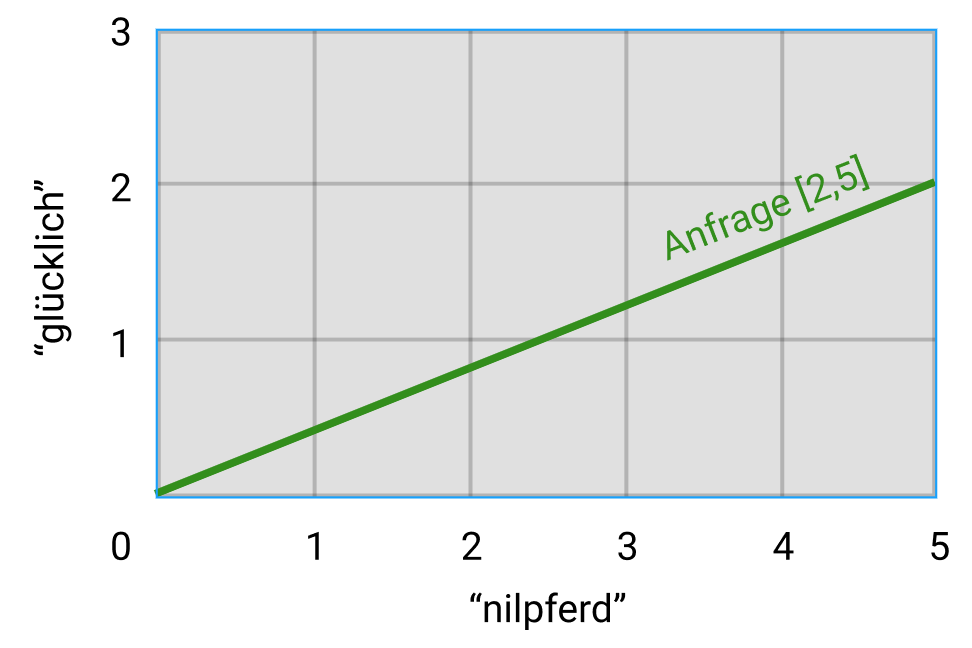
\includegraphics[scale=0.35]{assets/Diagram_1} \\
	Das gezeigte Koordinatensystem stellt den Vektor der Suchanfrage nach den Termen \texttt{glücklich} und \texttt{nilpferd} grafisch dar (Gormley und Tong 2015: 280).
\end{figure}

Der nächste Schritt umfasst das Erstellen ähnlicher Vektoren für jedes Dokument, bestehend aus den Gewichtungen der Terme \texttt{glücklich} und \texttt{nilpferd} im Kontext der individuellen Dokumente. \\

\begin{table}[htb]
	\centering
	\caption{Imaginäre Gewichtungen von imaginären Termen zur Darstellung in einem Beispiel}
	\begin{center}
		
		\begin{tabular}{| c | c | c |}
			\hline
			Dokument & Vorkommende Terme & Vektor mit Gewichtungen \\ [0.5ex]
			\hline \hline
			Dokument 1 & glücklich & [2,0] \\
			\hline
			Dokument 2 & nilpferd & [0,5] \\
			\hline
			Dokument 3 & glücklich, nilpferd & [2,5] \\
			\hline
		\end{tabular}
	\end{center}
	Die Tabelle zeigt imaginäre Gewichtungen zu beispielhaften Werten (Gormley und Tong 2015: 281).
\end{table} 

Werden diese Vektoren nun ebenfalls grafisch in einem Koordinatensystem dargestellt, entsteht folgende Abbildung.

\begin{figure}[h!]
	\centering
	\caption{Beispielhafte Darstellung mehrerer Vektoren zur imaginären Suche}
	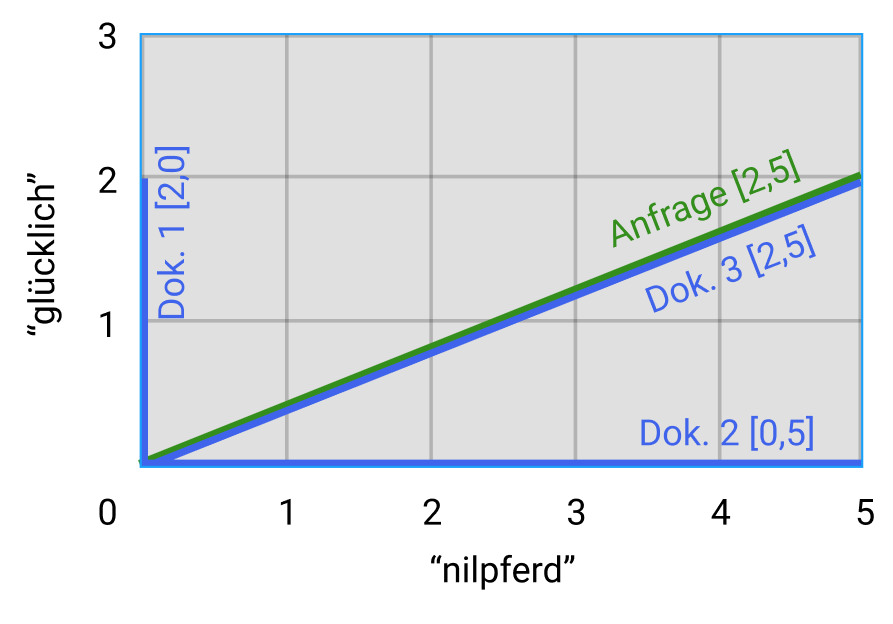
\includegraphics[scale=0.35]{assets/Diagram_2} \\
	Das gezeigte Koordinatensystem stellt Vektoren zu der Suche nach den Termen \texttt{glücklich} und \texttt{nilpferd} zusammen mit den Gewichtungen zu diesen Termen der einzelnen Dokumente grafisch dar.
\end{figure}

Diese Vektoren können nun miteinander verglichen werden. Dokument 3 hat in diesem Beispiel einen perfekten Treffer und erhält somit den höchsten Score. Vergleicht man die Graphen von Dokument 1 und Dokument 2 mit dem Graphen der Anfrage, fällt auf, dass der Winkel zwischen dem Graph der Anfrage und dem Graph von Dokument 2 sehr flach ist. Der Score von Dokument 2 ist demnach höher, als der von Dokument 3 (Gormley und Tong 2015: 281). \\
Dieses Beispiel beruht auf zwei Suchtermen, demnach sind die Vektoren zweidimensional und lassen sich ohne Weiteres zeichnen und vergleichen. Bei komplexeren Anfragen werden mehrdimensionale Vektoren erzeigt, welche mit linearer Algebra verglichen werden können (Gormley und Tong 2015: 281).

\section{Umsetzung}

\subsection{Idee}
Die Idee für dieses Projekt entstand bei der Suche nach weiterbildender Literatur zum Thema MongoDB in stadt.werks Library-Repository. Auch wenn die Bücher nach ihrem Titel sortiert waren, stellte es sich dennoch als mühselig heraus, jedes einzelne Buch als PDF herunterzuladen, zu öffnen und nach dem Begriff MongoDB zu durchsuchen. Um dieses Problem für alle Mitarbeiterinnen und Mitarbeiter von stadt.werk zu lösen, wurde folgende Idee formuliert.

\begin{center}
	Es soll eine Möglichkeit geschaffen werden, mithilfe moderner Webtechnologien die digitale Bibliothek nach Schlagworten und Begriffen zu durchsuchen und dem Nutzer die Treffer mit Angabe der Seite zurückzugeben.
\end{center}

Dieses Projekt stellte sich nach Vorstellung im Kollegium als gute Übung heraus. Jedoch erwies es sich nach Berücksichtigung der Aspekte Frontend, Backend und Datenhaltung als ein äußerst umfangreiches Projekt. Daher wird im Kontext dieser Arbeit lediglich ein Ausschnitt gezeigt, wobei zu berücksichtigen ist, dass die Arbeit an dem Projekt über den Rahmen dieser Arbeit hinaus weitergeführt wird. \\
Um die Wahl von Elasticsearch als zentrales Element dieses Projektes im Späteren zu begründen, wird die Performanz, mit welcher die Elasticsearch Treffer auf verknüpfte Anfragen findet, dargestellt.

\subsection{Elasticsearch für Projekte}
Die bekanntesten Einsatzgebiete von Elasticsearch wurden zu Beginn dieser Arbeit bereits erwähnt. Zieht man in Betracht, dass die Technologie kostenlos erhältlich ist, wird der Wert für Unternehmen jeder Größe, aber auch für Entwicklerinnen und Entwickler mit persönlichen Projekten, deutlich. Die Möglichkeit, eine Suchmaschine mit Volltextsuchfunktion und akzeptablen Systemvoraussetzungen auf einem Notebook, einem Desktopcomputer, einem Server, einem RaspberryPi oder sogar auf einem Smartphone funktional arbeiten zu lassen, ermöglicht und vereinfacht die Umsetzung vieler Projekte. Angenommen, der zentrale Zweck einer Software ist nicht das Durchsuchen von Daten, sondern das Zeigen von Videoinhalten. Sollte der Bedarf bestehen, den potenziell riesigen Umfang aller Videoinhalte einer Plattform zu durchsuchen, ist Elasticsearch für ein solches Projekt eine perfekte Ergänzung. Es lässt sich demnach sagen, dass Elasticsearch nicht zuletzt aufgrund der akzeptablen Systemvoraussetzungen nicht nur eine zentrale Rolle, wie in diesem Projekt, belegen muss, sondern aufgrund seiner Modularität ebenfalls als Zusatz zu bestehenden Projekten genutzt werden kann.

\subsection{Wahl der Technologien}
Die Wahl der für dieses Projekt zu verwendenden Technologien entstand aus dem Alltag bei stadt.werk. Jede der genutzten Technologien findet im Kontext der Arbeit bei stadt.werk Anwendung. Demnach konnte das Kollegium bei Fragen und Problemen gut helfen. Die Spezifikationen des Systems, auf welchem das Projekt erstellt wird, können folgender Tabelle entnommen werden.

\begin{table}[htb]
	\centering
	\caption{Systemkonfiguration des Hostsystems für das Projekt}
	\begin{center}
		
		\begin{tabular}{| c | c |}
			\hline
			Aspekt & System \\ [0.5ex]
			\hline \hline
			Modell & MacBook Pro (13 Zoll, 2020) \\
			\hline
			Prozessor & 2 GHz Quad-Core Intel Core i5 \\
			\hline
			Arbeitsspeicher & 32 GB 3733 MHz LPDDR4X \\
			\hline
			Betriebssystem & macOS Big Sur Version 11.2.3 \\
			\hline
		\end{tabular}
	\end{center}
	Die Tabelle zeigt die verwendete Hardware und das Betriebssystem zur Umsetzung des Projekts.
\end{table} 

Im Folgenden werden die verwendeten Technologien erläutert. Zusätzlich werden in Betracht gezogene Alternativen erwähnt. Dazu wird erläutert, warum diese Alternativen nicht genutzt werden.

\subsubsection{Node.js}
Node.js ist eine Laufzeitumgebung, die es ermöglicht, JavaScript außerhalb des Webbrowsers auszuführen. Die Laufzeitumgebung baut auf der V8 JavaScript Engine des Browsers Google Chrome auf. \\
Die Wahl von Node.js als Umgebung für das Projekt hat mehrere Gründe. Node.js ist die bei stadt.werk am häufigsten genutzte Technologie zur Umsetzung von Projekten. So baut die Umsetzung dieses Projektes auf bereits vorhandenes Wissen auf, vertieft dieses und ermöglicht weiteres Festigen von Theorie durch Praxis. Es bleibt zu erwähnen, dass ein Projekt auf der Basis von Node.js vorbereitend auf den Inhalt des vierten Semesters an der DHSH wirkt. \\

Eine wachsende Alternative zu Node.js bildet Deno. Deno nutzt ebenfalls die eingangs erwähnte JavaScript V8 Engine, wurde in der Programmiersprache Rust entwickelt und unterstützt nativ sowohl JavaScript als auch TypeScript. Die Wahl fällt schlussendlich auf Node.js, da Deno im Kontext von stadt.werk bisher keine Anwendung findet und Deno aufgrund des recht jungen Alters über wenige Erfahrungsberichte und wenig Dokumentation verfügt.

\subsubsection{JavaScript}
JavaScript ist eine Programmiersprache, welche in erster Linie Anwendung im Web findet. Durch Node.js oder Deno entsteht die Möglichkeit, in JavaScript geschriebene Programme als Serversoftware auszuführen. \\
Die Programmiersprache JavaScript findet im Kontext dieser Arbeit Anwendung, da viele Anwendungen von stadt.werk ebenfalls in JavaScript geschrieben werden. Weiterhin spielen bei der Wahl von Programmiersprachen natürlich immer die persönliche Präferenzen eine Rolle, so auch in diesem Fall. \\

Bei dem Vergleich mit Alternativen zu JavaScipt muss zwischen zwei Kategorien unterschieden werden. In der ersten Kategorie ist TypeScript einzuordnen, die zweite Kategorie wird von allen anderen existierenden Programmiersprachen gefüllt. TypeScript kann als eine Art Weiterentwicklung von JavaScript verstanden werden. Es werden beispielsweise Möglichkeiten zur Sicherstellung der Typsicherheit bereitgestellt, der Syntax von TypeScript dem von JavaScript sehr ähnlich. Nach Rücksprache mit dem Kollegium wird auf die Nutzung von TypeScript verzichtet, da dieses Projekt auf externen npm-Paketen beruht. Das würde bedeuten, dass für diese fremden Pakete zusätzliche Typendeklarationen geschrieben werden müssen, was wiederum den Rahmen des Projektes überschreiten würde und demnach mehr Nachteile als Vorteile bietet. \\
Die Kategorie aller anderen Programmiersprachen findet ebenfalls aus persönlicher Präferenz und aufgrund eines erzielten Lerneffekts für das Unternehmen keine Anwendung.

\subsubsection{npm}
Der Paketmanager npm für Node.js bietet die Möglichkeit, fremden quelloffenen Code in Form von Paketen zu nutzen. Er wird zusammen mit Node.js installiert und bietet eine Vielzahl von Paketen für verschiedenste Anwendungsbereiche.\\
Der Dienst npm wird als logische Schlussfolgerung zur Nutzung von Node.js gewählt. In den Projekt werden die folgenden Pakete genutzt.

\paragraph{elasticsearch}
Das Paket elasticsearch ist von Elasticsearch bereitgestellte Software zur Kommunikation mit einer Elasticsearch-Instanz im Syntax von JavaScript. \\
Alternativ zur Nutzung dieses Paketes kann das Ausschreiben von vollständigen HTTP-Anfragen gegen die Elasticsearch-APIs zurückgegriffen werden. Da die Nutzung des Paketes jedoch einfacher und unkomplizierter ist, wird auf das Ausformulieren von HTTP-Anfragen verzichtet.

\paragraph{pdf-parse}
Das Paket pdf-parse bietet neben zahlreichen anderen Aspekten die Möglichkeit, die Anzahl der Seiten einer PDF-Datei auszugeben. Der Nutzen dessen und welchen Vorteil das Paket bei der Umsetzung bringt, wird im Späteren erläutert.

\paragraph{mighty-pdf-parser}
Das Paket mighty-pdf-parser bietet die Möglichkeit, den Text von PDF-Dateien zu extrahieren und als Strings zu behandeln. Weiterhin bietet das Paket Parameter, mit welchen eingestellt werden kann, von welcher Seite einer PDF-Datei der Text als String extrahiert werden soll. Die Software basiert auf PDF.js, einer ausgereiften Software zum Behandeln von PDF-Dateien. \\
Die bekannteste Alternative zu mighty-pdf-parser und demnach auch PDF.js ist Apache Tika. Apache Tika ist ein in Java geschriebenes Werkzeug zur Extraktion von Text, Anhängen und Metadaten unzähliger Formate, darunter auch PDF. Bei der Umsetzung des Projektes wird sich aus mehreren Gründen gegen Apache Tika entschieden. Die Software ist, anders als das Projekt, in der Sprache Java geschrieben. Das würde bedeuten, dass ein separater Container mit einer Java-Umgebung und einem Apache Tika-Server erstellt werden muss. Das würde zusätzliche Rechenlast für das Hostsystem bedeuten. Weiterhin bietet Apache Tika keine Möglichkeit, individuelle Seiten in Text umzuwandeln. Das eingelesene Dokument wird im Ganzen zu einem String, einem JSON- oder einem XML-Objekt umgewandelt, bei Bedarf inklusive Metadaten. Um dem Nutzer zukünftig die Seite, welche den Suchtreffer enthält, auszugeben, muss das Programm eine Möglichkeit bieten, Seiten individuell umzuwandeln. Zuletzt bleibt zu erwähnen, dass Apache Tika für das einfache Extrahieren von Text aus PDF-Dateien zu umfangreich ist. Für diesen Fall lohnt es sich nicht, ein Werkzeug in diesem Umfang zu nutzen.

\subsubsection{Docker}
Um das Projekt auf jedem System starten zu können, wird Docker zur Virtualisierung von Containern genutzt. So kann Software mit allen nötigen Komponenten gebündelt und auf verschiedensten Systemen genutzt werden. Weiterhin besteht dank Docker die Möglichkeit, den Software-Stack nach Bedarf komponentenweise zu starten. Container zur Visualisierung müssen beispielsweise nicht gestartet werden, um Arbeiten an der Anwendungslogik vorzunehmen. Dies schont Ressourcen und hält das Hostsystem performant. \\
Die Entscheidung, Docker für dieses Projekt zu nutzen, hat mehrere Gründe. Dank der Virtualisierung von Containern wird ein kleinster gemeinsamer Nenner zwischen den Entwicklersystemen des Kollegiums geschaffen. Diese laufen je nach Präferenz auf anderen Betriebssystemen. So kann sicher gestellt werden, dass das Projekt überall lauffähig ist. Weiterhin bietet Docker einsatzbereite Images von Elasticsearch und Kibana an. So wird der technische Aufwand und potentielle Probleme mit der Infrastruktur des Projekts minimiert. Zuletzt bleibt zu erwähnen, dass die Arbeit bei stadt.werk einen guten Umgang mit Docker voraussetzt. Das Projekt ist demnach im Kontext der täglichen Arbeit eine gute Übung. \\

Da es kaum nennenswerte Alternativen zu Docker gibt, fällt die Entscheidung leicht. Dennoch seinen Virtualisierungsassistenten, wie VM-Ware oder Hyper-V erwähnt, welche jedoch zu umfangreich für ein Projekt dieser Größe scheinen.

\subsubsection{Elasticsearch}
Elasticsearch ist ein dokumentenorientiertes Datenbanksystem mit der Fähigkeit, Einträge zu indexieren und zu durchsuchen. Elasticsearch wird im Kontext von stadt.werk noch nicht lange genutzt, daher erscheint eine Einarbeitung in das Thema sinnvoll und zukunftsorientiert. \\
Über die Vorteile von Elasticsearch wird im Theorieteil dieser Arbeit bereits berichtet, daher sei hier lediglich erwähnt, dass Elasticsearch die bekannteste Technologie im Bereich Volltextsuchmaschinen ist. Elasticsearch ist kostenlos und quelloffen, was die Wahl weiterhin bestätigt.

\subsubsection{Kibana}
Elasticsearch allein ist optimiert für den serverseitigen Betrieb. Es wird keine grafische Oberfläche bereitgestellt, die Kommunikation erfolgt lediglich über die APIs. Kibana füllt diese Lücke und bietet eine grafische Oberfläche für Elasticsearch. Hier können zahlreiche Informationen zum Zustand der Datenbank eingesehen, sowie Logs ausgelesen werden. Die primäre Nutzung von Kibana erfolgt zum schnellen Testen von Anfragen gegen Elasticsearch. Das grafische Interface von Kibana erlaubt es einem Entwickler, schnell und einfach sogar komplexe Anfragen zu stellen und die Treffer zusammen mit der Geschwindigkeit direkt im Interface einzusehen. \\
Da Kibana von den Entwicklern von Elasticsearch stammt, fiel die Wahl schnell auf Kibana. Es müssen kaum Konfigurationen vorgenommen werden, die Nutzung erfolgt ohne Probleme.

\subsubsection{Postman}
Postman ist ein Programm zum Erstellen von HTTP-Anfragen und Testen von APIs. Es bietet eine grafische Oberfläche und Möglichkeiten zum Sichern von Zugangsdaten oder Cookies. Die Nutzung von Postman im Kontext dieser Arbeit liegt in dem anfänglich schnellen Testen, ob der Software-Stack hochgefahren ist, begründet. Im Verlauf der Arbeit wird auf das Benutzen von Kibana umgestellt und Postman findet keine Anwendung mehr. \\

Eine bekannte Alternative zu Postman bildet das Commandline-Werkzeug cURL. Es ist ein textbasiertes Programm zum Ausführen von HTTP-Anfragen und wird aufgrund von komplexeren Anfragen erst durch Postman, später durch Kibana ersetzt.

\subsubsection{Visual Studio Code}
Visual Studio Code ist eine Entwicklungsumgebung zum Entwickeln von Programmen. Der Texteditor bietet Syntaxhervorhebung für eine Vielzahl von Sprachen. Viele Mitarbeiterinnen und Mitarbeiter von stadt.werk nutzen Visual Studio Code. Auch hier sei erwähnt, dass die Wahl der Entwicklungsumgebung ein subjektives Thema ist, welches jedoch für den Betrieb des Projekts keine Relevanz besitzt. \\

Als Alternativen zu Visual Studio Code lassen sich die Produkte von JetBrains aufführen, aber auch Sublime oder Vim zählen zu dieser Kategorie.

\subsection{Schwierigkeiten}
Die Durchführung des Projekts bestand zu großen Teilen aus Recherche, Testen, Verwerfen von Ansätzen, Lernen und Anwenden neuer Technologien. \\
Beginnend mit dem Finden einer Technologie zum Auslesen von Text aus PDF-Dateien lässt sich sagen, dass sehr viel Zeit in das Evaluieren und Experimentieren mit Apache Tika geflossen ist. Es wurde versucht, Apache Tika mit Parametern zu versehen, den Quellcode anzupassen oder ein Plugin für Elasticsearch zu verwenden, welches auf Apache Tika basiert. Letztendlich erwies sich der ständige Wechsel zwischen Java und JavaScript als Herausforderung und Apache Tika wurde, nicht zuletzt aufgrund der Vorteile von mighty-pdf-parser, verworfen. Nach dem Evaluieren und Testen mehrerer npm-Pakete, fiel die Wahl auf mighty-pdf-parser und pdf-parse aus den bereits beschriebenen Gründen. \\
Weitere Schwierigkeiten traten im Kontext von Docker auf. Die erstellten Container mussten mittels Docker-Compose einem gemeinsamen Netzwerk zugeordnet werden, um untereinander Kommunizieren zu können. \\
Dank der täglichen Arbeit bei stadt.werk und der Expertise des Kollegiums konnten viele Fehler schnell gelöst werden.
    
\subsection{Ergebnis der Umsetzung}
Vorab sei erwähnt, dass sich im Anhang ein Link zu einem öffentlichen Git Repository befindet. Während der erstellte Quellcode öffentlich einsehbar ist, bildet die digitale Bibliothek ein privates Submodul in diesem Repository und kann aus Gründen der Lizenzierung nicht öffentlich gemacht werden. Sollte Interesse an einer Einsicht auf die Bibliothek bestehen, wird darum gebeten, dies im Speziellen zu erfragen. \\

Im Folgenden wird die Infrastruktur, sowie die Abläufe in der verwendeten und erstellten Software aufgezeigt. Die höchste Schicht bilden die Docker-Container. Es existiert je ein Container für Elasticsearch, Kibana und die Anwendungslogik. Die Images für Elasticsearch und Kibana stammen von den Entwicklern von Elasticsearch und sind frei zugänglich, das Image für die Anwendungslogik wird selbst gebaut. Wie bereits erwähnt basiert die Anwendungslogik auf Node.js und ist in der Sprache JavaScript geschrieben. Der Container für die Anwendungslogik enthält ebenfalls die digitale Bibliothek in Form eines Git Submodules. Die digitale Bibliothek enthält 141 Bücher in Form von PDF-Dateien. \\

Um diese in Elasticsearch zu übertragen, wird zunächst ein Index und ein Typ mit dem Namen library und book erstellt. Um den Typ in einem ersten Schritt mit Dokumenten zu füllen, wird über jede PDF-Datei iteriert und für jedes Buch wird ein Dokument angelegt. Jedes Dokument enthält zu diesem Zeitpunkt nur eine ID mit dem Titel des Buchs, sowie ein Feld documentName, in welchem ebenfalls der Titel gesichert wird. \\
Wird dieser Schritt erfolgreich abgeschlossen, iteriert die Anwendungslogik in einem zweiten Schritt über jede PDF-Datei. Für jede PDF-Datei wird mithilfe des npm-Pakets pdf-parse die Anzahl der Seiten gesichert. Mithilfe des npm-Pakets mighty-pdf-parser wird nun über jede Seite des Buchs iteriert und der Inhalt wird in einer Liste von Strings gesichert. Ist die Iteration über jede Seite eines Buchs abgeschlossen, wird die Liste von Strings mit dem Titel des Buchs an den Elasticsearch-Client übergeben. Dieser aktualisiert das zugehörige Dokument in Elasticsearch mit der Liste in dem Feld documentContent. Sobald alle Bücher und deren Inhalte in Text umgewandelt und indexiert wurden, kann mithilfe von Kibana eine einfache Suchanfrage erstellt werden, die alle Dokumente des Indexes zurückgibt. So kann händisch überprüft werden, ob das Indexieren funktioniert hat. Der Docker-Container mit der Anwendungslogik hat für weiteres Testen keinen Nutzen mehr und fährt nach erfolgreicher Indexierung herunter. Es verbleiben noch die Container für Elasticsearch und Kibana. Im Kontext dieser Arbeit wird Kibana genutzt, um die Geschwindigkeit von Elasticsearch bei komplexen Anfragen darzustellen.

\subsection{Überprüfung der aufgestellten Theorie}
Der Nutzen von einer digitalen Bibliothek in Kombination mit einer Volltextsuchmaschine wurde bereits erläutert. Um die Geschwindigkeit dieser darzustellen, wurden komplexe, über logische Ausdrücke verknüpfte Suchanfragen erstellt und 50 mal pro Anfrage durchgeführt. Es ist zu berücksichtigen, dass die Anfragen in der englischen Sprache verfasst wurden, da die indexierte Literatur ebenfalls ausschließlich auf Englisch vorliegt:

\begin{itemize}
	\item 'database'
	\item 'relational'$\land$'database'
	\item ('relational'$\land$'database')$\neg$'sql'
	\item ('game'$\land$'development'$\land$'ios')$\neg$'android'
	\item ('game'$\land$'development'$\land$'unity')$\neg$'unreal'$\neg$'android'$\neg$'ios'
	\item ('html'$\land$'css')$\neg$'javascript'
	\item ('php'$\land$'api'$\land$'server')$\neg$'java'$\neg$'javascript'
	\item 'git'$\land$'python'
	\item 'jquery'$\neg$'javascript'
	\item ('html'$\land$'css'$\land$'javascript')$\neg$'framework'
\end{itemize}

Die Geschwindigkeit von Elasticsearch wird mithilfe des Felds took ermittelt. Es zeigt eine Zahl vom Typ Integer, welche die benötigte Zeit in Millisekunden darstellt. Von den 50 Anfragen pro Anfragekonstrukt wird die Zahl der gefundenen Dokumente und die mittlere Geschwindigkeit festgehalten.

\newpage

\section{Ergebnisse}
Die vollständige Tabelle mit allen Zahlen sind im Anhang zu finden. Die mittlere Geschwindigkeit und die Menge der Treffer für jedes Anfragekonstrukt wird in folgender Tabelle zusammengefasst.

\begin{table}[htb]
	\centering
	\caption{Ergebnisse Performanztest Elasticsearch}
	\begin{center}
		
		\begin{tabular}{| l | l | l |}
			\hline
			Anfrage & Anzahl Treffer & \makecell[l]{Durchschnittliche Dauer \\ (auf ganze Zahlen gerundet)} \\ [0.5ex]
			\hline \hline
			'database' & 98 Treffer & 46ms \\
			\hline
			'relational'$\land$'database' & 28 Treffer & 53ms \\
			\hline
			('relational'$\land$'database')$\neg$'sql' & 08 Treffer & 28ms \\
			\hline
			\makecell[l]{('game'$\land$'development'$\land$'ios') \\ $\neg$'android'} & 11 Treffer & 39ms \\
			\hline
			\makecell[l]{('game'$\land$'development'$\land$'unity') \\ $\neg$'unreal'$\neg$'android'$\neg$'ios'} & 03 Treffer & 20ms \\
			\hline
			('html'$\land$'css')$\neg$'javascript' & 02 Treffer & 16ms \\
			\hline
			\makecell[l]{('php'$\land$'api'$\land$'server') \\ $\neg$'java'$\neg$'javascript'} & 00 Treffer & 1ms \\
			\hline
			'git'$\land$'python' & 29 Treffer & 44ms \\
			\hline
			'jquery'$\neg$'javascript' & 01 Treffer & 14ms \\
			\hline
			\makecell[l]{('html'$\land$'css'$\land$'javascript') \\ $\neg$'framework'} & 04 Treffer & 23ms\\
			\hline
		\end{tabular}
	\end{center}
	Die Tabelle zeigt die logisch verknüpften Anfragen, die Anzahl der Treffer und die mittlere Zeit, die Elasticsearch für die Rückgabe der Treffer benötigt. Die vollständige Tabelle findet sich im Anhang dieser Arbeit.
\end{table} 

\newpage

\section{Fazit}
Die Motivation hinter dieser Arbeit besteht aus der Erstellung einer neuen Software für das Ausbildungsunternehmen stadt.werk. Die Software sollte dabei die bisherige digitale Bibliothek um die Funktion einer bücherübergeifenden Volltextsuche erweitern. Dieses Ziel gilt mit dem Abschluss dieser Arbeit erreicht, wobei das Projekt zukünftig ausgebaut wird. \\
Die Menschheit befindet sich mitten im Zeitalter der Informationsexplosion. Es ist davon auszugehen, dass die Vielzahl von Informationen, Daten und Wissen, die tagtäglich generiert wird und in Unmengen auf die Menschen einprasselt, nicht weniger wird. Daher wird es täglich wichtiger, diese Daten und Informationen gut sortiert einfach zugänglich zu machen. Gerade im Bereich von Unternehmen kann ein Aufschieben dieser Tätigkeit schnell zu einem gewaltigen Berg von Arbeit führen, den es früher oder später aufzuholen gilt. \\
Diese Arbeit zeigt an einem praxisnahen Beispiel, wie mithilfe von kostenfreien Technologien ein hiermit nachgewiesenermaßen performantes System zum Durchsuchen von Informationen aller Art geschaffen werden kann. \\

Die erhobenen Daten zeigen beispielhaft, wie mithilfe von Elasticsearch aus tausenden Seiten Wissen, hunderte Seiten relevanter Information gewonnen werden kann. Dies geschieht innerhalb von Bruchteilen einer Sekunde. Die Möglichkeiten, diese Geschwindigkeit in einem noch größeren Kontext zu nutzen, scheinen endlos. 

\newpage

\section{Methodik}
Diese Arbeit wurde nicht mit der Intension geschrieben, eine nicht existente Software zu schaffen. Ganz im Gegenteil, die Vorteile, die Nachteile und die Nutzung von Elasticsearch sind vielfach dokumentiert. Die Messung der Performanz von Elasticsearch verfolgt in diesem Kontext keinen statistischen Zweck. Sie soll lediglich zeigen, wozu die verwendeten Technologien in der Lage sind. \\

Es bleibt jedoch zu kritisieren, dass die verwendeten npm-Pakete seit langem keine Updates erhielten. Weiterhin muss kritisiert werden, dass obwohl das erschaffene Programm quelloffen ist, die Bibliothek leider nicht eingesehen werden kann. Dies ist in erster Linie aufgrund der Lizenzmodelle der Literatur nicht ohne weiteres möglich.

% ---------------------
% Literaturverzeichnis:
% ---------------------

% Neue Seite beginnen:
\newpage

% Seitenzahl als römische Zahl angeben:
\pagenumbering{Roman}

% Beginn der Zählung bei 5:
\setcounter{page}{6}

% Literaturverzeichnis zu TOC hinzufügen:
\addcontentsline{toc}{section}{Liteaturverzeichnis}

% Literaturverzeichnis:
\section*{Literaturverzeichnis}

% Einfacher Zeilenabstand:
\singlespacing

Alsop, T. (2020): \textit{Global hard disk drive (HDD) shipments 1976-2025}, [online] \\ \href{https://www.statista.com/statistics/398951/global-shipment-figures-for-hard-disk-drives/}{https://www.statista.com/statistics/398951/global-shipment-figures-for-hard- \\ disk-drives/}, statista, (09.04.2021) \\ \\
Benlian, A. und Hess, T. (2011): \textit{Opportunities and risks of software-as-a-service: Findings from a survey of IT executives}, Decision Support Systems, Nr. 52, S. 232 - 246 \\ \\
\textit{Configure security for the Elastic Stack} (o.D.), [online] \href{https://www.elastic.co/guide/en/elasticsearch/reference/current/configuring-stack-security.html}{https://www.elastic.co/guide/ \\ en/elasticsearch/reference/current/configuring-stack-security.html}, elastic, \\ (10.04.2021) \\ \\
Decker, B. und Finke, I. und John, M. und Joisten, M. und Schnalzer, K. und Voigt, S. und Wesoly, M. und Will, M. (2015): \textit{Wissen und Information 2005}, Fraunhofer IRB Verlag, Stuttgart \\ \\
Deacon, J. (2009): \textit{Model-View-Controller (MVC) Architecture}, JOHN DEACON Computer Systems Development, Consulting \& Training \\ \\
\textit{Elasticsearch Node.js client} (o.D.), [online] \href{https://www.elastic.co/guide/en/elasticsearch/client/javascript-api/current/index.html}{https://www.elastic.co/guide/en/ \\ elasticsearch/client/javascript-api/current/index.html}, elastic, (10.04.2021) \\ \\
EU-Kommission (2013): \textit{EMPFEHLUNG DER KOMMISSION vom 6. Mai 2003 betreffend die Definition der Kleinstunternehmen sowie der kleinen und mittleren Unternehmen}, Bekannt gegeben unter Aktenzeichen K(2003) 1422, 2003/361/EG \\ \\
Gormley, C. und Tong, Z. (2015): \textit{Elasticsearch - The Definitive Guide}, O'Reilly Media, Sebastopol \\ \\
\textit{Ihr Fenster in den Elastic Stack} (o.D.), [online] \href{https://www.elastic.co/de/kibana}{https://www.elastic.co/de/kibana}, elastic, (12.04.2021) \\ \\
\textit{Kibana Query Language} (o.D.), [online] \href{https://www.elastic.co/guide/en/kibana/7.9/kuery-query.html}{https://www.elastic.co/guide/en/kibana/7.9/ \\ kuery-query.html}, elastic, 12.04.2021 \\ \\
Meier, A. und Kaufmann, M. (2016): \textit{SQL- \& NoSQL-Datenbanken}, Springer Vieweg, Berlin Heidelberg \\ \\
Moore, K. (2000): \textit{The Ancient Art of Knowledge Management}, Knowledge Management Review, Nr. 12 (Jan/Feb 2000), S. 12 - 13 \\ \\
Pezoa, F. und Reutter, J. L. und Suarez, F. und Ugarte, M. und Vrgoč, D. (2016): \textit{WWW '16: Proceedings of the 25th International Conference on World Wide Web}, (April 2016), S. 263 - 273 \\ \\
Probst, G. und Raub, S. und Romhardt, K. (2006): \textit{Wissen managen - Wie Unternehmen ihre wertvollste Ressource optimal nutzen}, GWV Fachverlage GmbH, Wiesbaden \\ \\
\textit{Similarity module} (o.D.), [online] \href{https://www.elastic.co/guide/en/elasticsearch/reference/current/index-modules-similarity.html}{https://www.elastic.co/guide/en/elasticsearch/ \\ reference/current/index-modules-similarity.html}, elastic, (09.04.2021) \\ \\
\textit{Was ist Elasticsearch?} (o.D.), [online] \href{https://www.elastic.co/de/what-is/elasticsearch/}{https://www.elastic.co/de/what-is/elasticsearch/}, elastic, (09.04.2021) \\ \\
\textit{What does tf-idf mean?} (o.D.), [online] \href{http://www.tfidf.com}{http://www.tfidf.com}, tfidf.com, (12.04.2021) \\ \\
Wöhe, G. und Döring, U. (2010): \textit{Einführung in die Allgemeine Betriebswirtschaftslehre}, Verlag Franz Vahlen GmbH, München \\ \\

% --------------------------
% Eidesstattliche Erklärung:
% --------------------------

% Neue Section:
\section*{Eidesstattliche Erklärung}

\addcontentsline{toc}{section}{Eidesstattliche Erklärung}

% 1,5-facher Zeilenabstand:
\onehalfspacing

Ich erkläre an Eides Statt, dass ich meine Hausarbeit „Der Nutzen von digitalem Wissensmanagement in mittelständischen IT-Unternehmen - am Beispiel einer digitalen Bibliothek“ selbstständig und ohne fremde Hilfe angefertigt habe und dass ich alle von anderen Autoren wörtlich übernommenen Stellen wie auch die sich an Gedankengänge anderer Autoren eng anlehnenden Ausführungen meiner Arbeit besonders gekennzeichnet und die Quelle nach den mir von der Dualen Hochschule Schleswig-Holstein angegebenen Richtlinien zitiert habe. \\ \\

Kiel, den 29.04.2021 \\ \\ 

% Tabbing-Umgebung für Unterschriften:
\begin{tabbing}
	\_\_\_\_\_\_\_\_\_\_\_\_\_\_\_\_\_\_\_\_\_\_\_\_\_ \\
	Fabian Reitz
\end{tabbing}

% -------
% Anhang:
% -------

% Neue Seite beginnen:
\newpage

\appendix
% Neue Section:
\section{Git Repository}
Das öffentliche Git Repository befindet sich auf GitHub und ist unter folgendem Link auffindbar: \href{https://github.com/FabianReitz/Praxisprojekt-2}{https://github.com/FabianReitz/Praxisprojekt-2}

\section{Vollständige Tabelle der Performanzmessung der Elasticsearch}

\begin{itemize}
	\item \textbf{query01:} 'database'
	\item \textbf{query02:} 'relational'$\land$'database'
	\item \textbf{query03:} ('relational'$\land$'database')$\neg$'sql'
	\item \textbf{query04:} ('game'$\land$'development'$\land$'ios')$\neg$'android'
	\item \textbf{query05:} ('game'$\land$'development'$\land$'unity')$\neg$'unreal'$\neg$'android'$\neg$'ios'
	\item \textbf{query06:} ('html'$\land$'css')$\neg$'javascript'
	\item \textbf{query07:} ('php'$\land$'api'$\land$'server')$\neg$'java'$\neg$'javascript'
	\item \textbf{query08:} 'git'$\land$'python'
	\item \textbf{query09:} 'jquery'$\neg$'javascript'
	\item \textbf{query10:} ('html'$\land$'css'$\land$'javascript')$\neg$'framework'
\end{itemize}
Die Werte sind in Millisekunden angegeben.

\begin{table}[htb]
	\centering
	\caption{Vollständige Ergebnisse Performanztest Elasticsearch}
	\begin{adjustwidth}{-2cm}{-2cm}
		
		\begin{tabular}{| l | l | l | l | l | l | l | l | l | l |}
			\hline
			query01 & query02 & query03 & query04 & query05 & query06 & query07 & query08 & query09 & query10 \\ [0.5ex]
			\hline \hline
			46 & 53 & 30 & 37 & 21 & 16 & 00 & 41 & 17 & 23 \\
			\hline
			41 & 59 & 32 & 40 & 16 & 18 & 00 & 43 & 10 & 21 \\
			\hline
			38 & 46 & 29 & 34 & 23 & 17 & 02 & 42 & 16 & 25 \\
			\hline
			45 & 50 & 27 & 39 & 25 & 10 & 01 & 41 & 15 & 13 \\
			\hline
			51 & 45 & 26 & 40 & 20 & 10 & 01 & 42 & 18 & 25 \\
			\hline
			43 & 50 & 31 & 36 & 25 & 21 & 02 & 50 & 15 & 20 \\
			\hline
			41 & 48 & 25 & 44 & 26 & 11 & 02 & 46 & 08 & 24 \\
			\hline
			45 & 61 & 24 & 36 & 19 & 10 & 02 & 41 & 20 & 26 \\
			\hline
			42 & 56 & 28 & 35 & 23 & 16 & 02 & 46 & 19 & 23 \\
			\hline
			45 & 51 & 30 & 40 & 15 & 22 & 01 & 50 & 12 & 25 \\
			\hline
			50 & 61 & 31 & 34 & 19 & 17 & 02 & 39 & 09 & 22 \\
			\hline
			37 & 44 & 32 & 43 & 24 & 16 & 01 & 49 & 18 & 23 \\
			\hline
			41 & 46 & 26 & 34 & 17 & 20 & 01 & 45 & 19 & 25 \\
			\hline
			39 & 41 & 28 & 36 & 26 & 22 & 01 & 50 & 16 & 20 \\
			\hline
			52 & 63 & 24 & 38 & 25 & 12 & 01 & 41 & 20 & 27 \\
			\hline
			53 & 58 & 29 & 42 & 25 & 20 & 00 & 48 & 09 & 26 \\
			\hline
			65 & 53 & 27 & 36 & 19 & 18 & 02 & 49 & 09 & 26 \\
			\hline
			45 & 57 & 25 & 43 & 26 & 18 & 02 & 42 & 21 & 25 \\
			\hline
			43 & 49 & 24 & 36 & 23 & 17 & 00 & 41 & 13 & 24 \\
			\hline
			42 & 52 & 25 & 40 & 22 & 13 & 02 & 42 & 12 & 21 \\
			\hline
			42 & 65 & 28 & 37 & 15 & 15 & 02 & 47 & 15 & 22 \\
			\hline
			45 & 59 & 27 & 41 & 16 & 20 & 00 & 47 & 19 & 26 \\
			\hline
			46 & 43 & 29 & 34 & 19 & 22 & 00 & 44 & 19 & 21 \\
			\hline
			48 & 60 & 32 & 44 & 24 & 20 & 00 & 45 & 09 & 21 \\
			\hline
			46 & 42 & 26 & 40 & 20 & 17 & 01 & 47 & 09 & 24 \\
			\hline
			47 & 54 & 31 & 34 & 16 & 10 & 02 & 38 & 14 & 27 \\
			\hline
			54 & 48 & 30 & 35 & 17 & 14 & 01 & 39 & 08 & 22 \\
			\hline
			57 & 64 & 32 & 38 & 16 & 11 & 00 & 43 & 13 & 19 \\
			\hline
			46 & 62 & 30 & 42 & 15 & 14 & 02 & 44 & 09 & 25 \\
			\hline
			43 & 45 & 26 & 37 & 18 & 09 & 01 & 48 & 11 & 20 \\
			\hline
			42 & 55 & 28 & 36 & 16 & 21 & 02 & 39 & 08 & 26 \\
			\hline
			44 & 47 & 24 & 40 & 15 & 21 & 02 & 49 & 13 & 26 \\
			\hline
			48 & 50 & 29 & 39 & 20 & 08 & 01 & 45 & 12 & 23 \\
			\hline
			45 & 55 & 27 & 42 & 17 & 19 & 00 & 45 & 16 & 23 \\
			\hline
			45 & 44 & 25 & 40 & 23 & 20 & 01 & 39 & 19 & 23 \\
			\hline
			47 & 46 & 31 & 43 & 17 & 17 & 00 & 38 & 20 & 20 \\
			\hline
			54 & 52 & 32 & 42 & 16 & 22 & 00 & 40 & 16 & 27 \\
			\hline
			38 & 47 & 24 & 37 & 23 & 10 & 00 & 43 & 09 & 20 \\
			\hline
			39 & 43 & 28 & 35 & 19 & 18 & 01 & 42 & 14 & 26 \\
			\hline
			51 & 63 & 27 & 43 & 23 & 11 & 02 & 43 & 16 & 24 \\
			\hline
			40 & 45 & 29 & 34 & 20 & 12 & 00 & 41 & 20 & 22 \\
			\hline
			48 & 57 & 30 & 44 & 20 & 20 & 00 & 47 & 10 & 22 \\
			\hline
			45 & 65 & 26 & 41 & 21 & 15 & 00 & 50 & 14 & 22 \\
			\hline
			56 & 60 & 31 & 39 & 26 & 12 & 02 & 45 & 10 & 26 \\
			\hline
			55 & 54 & 25 & 35 & 16 & 14 & 02 & 47 & 15 & 25 \\
			\hline
			57 & 58 & 24 & 43 & 15 & 20 & 02 & 39 & 14 & 21 \\
			\hline
			50 & 41 & 32 & 44 & 22 & 08 & 02 & 50 & 21 & 21 \\
			\hline
			37 & 51 & 27 & 44 & 22 & 08 & 01 & 46 & 21 & 26 \\
			\hline
			49 & 62 & 25 & 41 & 26 & 22 & 02 & 45 & 09 & 27 \\
			\hline
			53 & 53 & 29 & 37 & 20 & 20 & 01 & 47 & 15 & 22 \\ 
			\hline
		\end{tabular}
	\end{adjustwidth}
\end{table} 



\end{document}


















